\documentclass[12pt,letterpaper]{article}
\usepackage[utf8]{inputenc}
\usepackage{amsmath}
\usepackage{amsfonts}
\usepackage{amssymb}
\usepackage{pdfpages}
\usepackage[left=1in, right=1in, top=0.5in, bottom=1in]{geometry}
\title{ChessAce: Problem Statement}
\author{Team MIF(G18): Jerry Ke, Mengshan Cui, Harry Fu}
\date{}

\begin{document}
\maketitle
\section{Team meeting plan}
Team meeting shall happen every Tuesday, Wednesday in ITB 236, and Friday in Thode library. If it is necessary, an additional weekend meeting will be announced at least twenty-four hour ahead. The weekend meeting will be on either Saturday or Sunday based on discussion.\\
One dedicated person shall record the discussion topics, ideas, conflicts, and decision happen or made during the meeting. One dedicated person shall prepare the detailed agendas that need to discuss, place items in the order of priority and estimate real time of each topic. Roles can switch among the team members via discussion.\\

\section{Rules of agendas}
$\bullet$ Record of the meeting shall be kept till the end of the project development.\\
$\bullet$ Late attendance is forgivable if it is in 15 minutes after the decided meeting time. A warning should be given after 15 minutes but before 30 minutes. The second warning shall be recorded. Any late attendance after 30 minutes or a complete absence shall be recorded as well. If the late attendance or absence is caused by force majeure, then the recorded may be erased after discussion.\\
$\bullet$ All members have the responsibility to be physically and mentally present.\\
$\bullet$ All members have the responsibility to stop any irrational, emotional conflicts or personal attacks happen immediately during the meeting.\\
$\bullet$ Every meeting has to end with written statement or decision made. Leave ahead must come with a valid reason.\\
$\bullet$ At the end of the meeting, everyone should understand their deliverable for the next meeting.\\

\section{Team member roles}
$\bullet$ Team leader: Jerry Ke\\
$\bullet$ Software Developer: Harry Fu, Jerry Ke, Mengshan Cui\\
$\bullet$ Negotiator: Harry Fu\\
$\bullet$ Documentation: Mengshan Cui\\
$\bullet$ Revisor \& Latex Formatting: Jerry Ke, Mengshan Cui, Harry Fu\\
$\bullet$ Git Management: Harry Fu\\

\section{Team communication plan}
In-campus we will communicate face to face at Thode library to work together. Off-campus, we are going to use a social media application called “WeChat” to share all the work details, important files and talk about meeting time. If any particular situation happened first we will talk on WeChat if no one response we will use the phone call. All the documentation will be posted and edited on the Google doc then post a Latex version on Gitlab. All programming works will be posted and edited on the Gitlab, team members can access Gitlab and create branches to work on them.\\

\section{Git workflow plan}
The development of ChessMaster will happen on Gitlab. The origin/master branch will be the centralized branch which aims to stable code release. Right now, origin/develop and origin/release branch is necessary for the development. Develop branch should contain the evolving codes that are not stable enough. Release branch should provide the stable codes ready to merge back to master branch, but minor bug fixes may happen before actual release. At this point, September 28th, Git management will not consider Feature and Hotfix branch, since the structure and number of features of the project are not as sophisticated as most of the other MMO or RPG games. Team MIF will use tags to mark major document or code updates, which correspond to the milestones established at the beginning of the semester.\\

\section{Proof of concept demonstration plan}
Even though chess is a relative simple project to implement, there are still many existing risks that Team MIF has to overcome. Risks separates into two categories, which are implementation and tests. Implementation risk mainly associate with “attack-range” detection, which prevents king from suiciding. \\ 
Because there is no test implementation in the original ChessOOP project, we have to design all the test plans by ourselves. The hard part in software testing is we have to consider all expected output for our program. However, since chess involves tremendous amount of variety, it is never impossible to include all the scenarios.\\
To show the above risks can be overcomed, Team MIF plans to implement a preliminary prototype with fundamental functions with minimal bugs and complete chess functions. GUI may not be included in the first POC demonstration, but will be added later on.\\

\section{Technology}
$\bullet$ Programming language: based on Java\\
$\bullet$ IDE: Microsoft Visual Studio/Eclipse/Atom\\
$\bullet$ Development platform: Gitlab\\
$\bullet$ Work flow chart: GanttProject\\
$\bullet$ Documentation: Latex and PDF file\\
 
\section{Coding style}
The project will refer to Google Java Style with some changes. Tab character will be used instead of 2 or 4 spaces for indentation between continuation lines and contents of a block. Multiple variables will be permitted in one variable declaration (int a, b), and local variables will be declared at the start of their containing block or block-like construct, not declared when needed. Identifier expression may use special prefixes or suffixes which is not allowed in Google Java Style.\\

\section{Project schedule}
	Refer to ChessAce\_team18.gan/pdf under the same directory. Screenshots below.
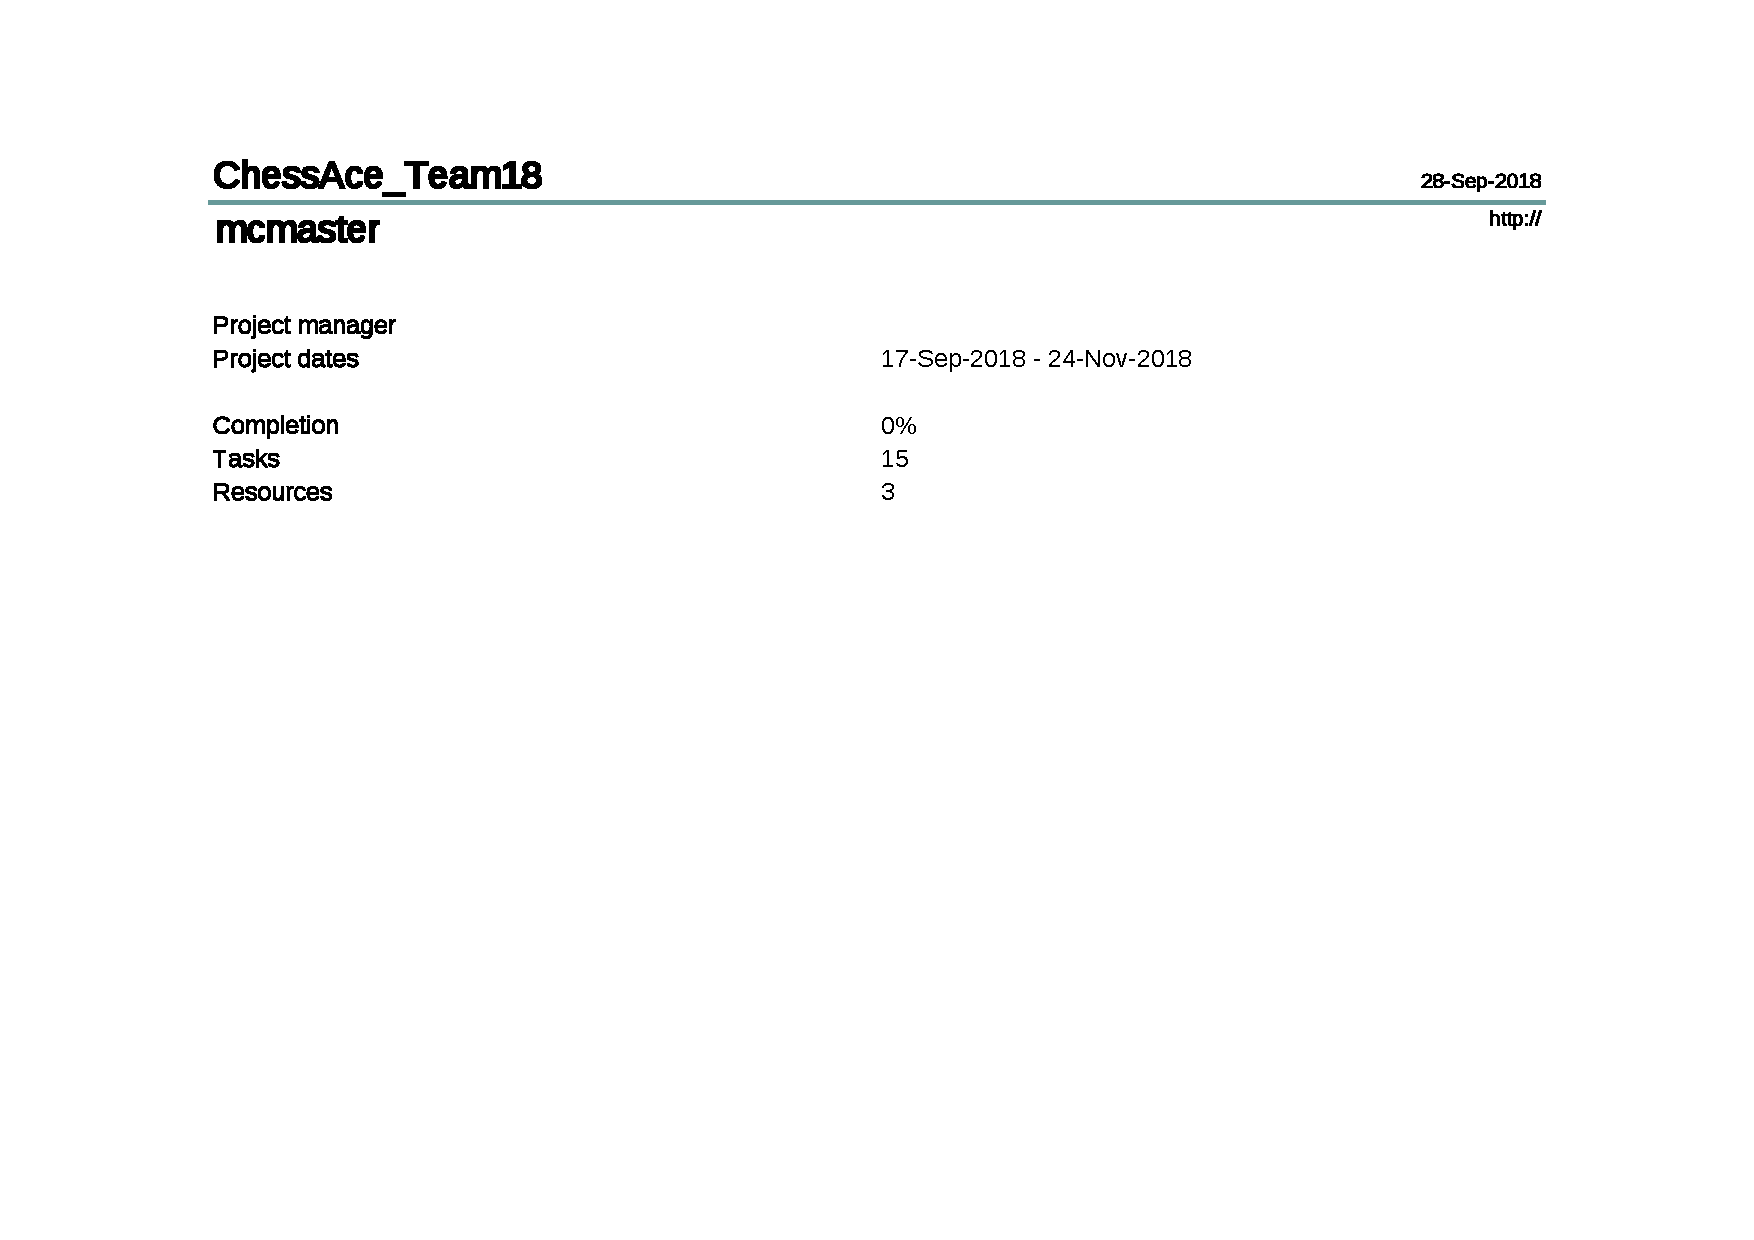
\includepdf[pages=-]{ChessAce_team18.pdf}

\section{Project review (for Revision 1)}
\end{document}